\chapter{Buttons and Serial Communications}
\chaplabel{buttons}

\section{Introduction}
This chapter introduces students to using buttons and serial communications.

\section{Types of Serial}

\begin{figure}[!htb]
	% Serial
	\begin{tikzpicture}
		% BLOCKS
		\draw[thick] (0,0) rectangle (4,4) node (dev1) [pos=0.5] {Device 1};
		\draw[thick] (8,0) rectangle (12,4) node (dev2) [pos=0.5] {Device 2};
		% ARROWS	
		\draw [thick,-{latex[length=4mm, width=6mm]}] (4,2) |- node [above,pos=0.75] {01101101} (8,2) ;
	\end{tikzpicture}
	\label{fig:serial}
	\caption{Serial transfers one bit at a time.}
\end{figure}
	
	% Parallel
\begin{figure}[!htb]
	\begin{tikzpicture}
		% BLOCKS
		\draw[thick] (0,0) rectangle (4,5) node (dev3) [pos=0.5] {Device 1};
		\draw[thick] (8,0) rectangle (12,5) node (dev4) [pos=0.5] {Device 2};
		% ARROWS	
		\draw [thick,-{latex[length=4mm, width=6mm]}] (4,4.25) |- node [above,pos=0.75] {0} (8,4.25) ;
		\draw [thick, -{latex[length=4mm, width=6mm]}] (4,3.75) |- node [above,pos=0.75] {1} (8,3.75) ;
		\draw [thick, -{latex[length=4mm, width=6mm]}] (4,3.25) |- node [above,pos=0.75] {1} (8,3.25) ;
		\draw [thick, -{latex[length=4mm, width=6mm]}] (4,2.75) |- node [above,pos=0.75] {0} (8,2.75) ;
		\draw [thick, -{latex[length=4mm, width=6mm]}] (4,2.25) |- node [above,pos=0.75] {1} (8,2.25) ;
		\draw [thick, -{latex[length=4mm, width=6mm]}] (4,1.75) |- node [above,pos=0.75] {1} (8,1.75) ;
		\draw [thick, -{latex[length=4mm, width=6mm]}] (4,1.25) |- node [above,pos=0.75] {0} (8,1.25) ;
		\draw [thick, -{latex[length=4mm, width=6mm]}] (4,0.75) |- node [above,pos=0.75] {1} (8,0.75) ;
		
	\end{tikzpicture}
	\label{fig:parallel}
	\caption{Parallel transfers multiple bits at a time.}
\end{figure}

\begin{figure}[!htb]
	% UART
	\begin{tikzpicture}
		% BLOCKS
		\draw[thick] (0,0) rectangle (4,4) node (dev1) [pos=0.5] {Device 1};
		\draw[thick] (8,0) rectangle (12,4) node (dev2) [pos=0.5] {Device 2};
		% ARROWS	
		\draw [thick,-{latex[length=4mm, width=6mm]}] (4,2.5) node [anchor=east] {TX} -- (8,1.5) node [anchor=west] {RX} ;
		\draw [thick,{latex[length=4mm, width=6mm]}-] (4,1.5) node [anchor=east] {RX} -- (8,2.5) node [anchor=west] {TX} ;
	\end{tikzpicture}
	\label{fig:uart}
	\caption{A UART has full duplex between two entities.}
\end{figure}

\begin{figure}[!htb]
	% SPI
	\begin{tikzpicture}
		% BLOCKS
		\draw[thick] (0,0) rectangle (4,4) node (dev1) [pos=0.5] {Controller};
		\draw[thick] (8,0) rectangle (12,4) node (dev2) [pos=0.5] {Peripheral 1};
		\draw[thick] (8, -2) rectangle (12,-6) node (dev3) [pos=0.5] {Peripheral 2};
		% ARROWS	
		\draw [thick,-{latex[length=4mm, width=6mm]}] (4,2.5) node [anchor=east] {COPI} -- (8,2.5) node [anchor=west] {COPI} ;
		\draw [thick,{latex[length=4mm, width=6mm]}-] (4,1.5) node [anchor=east] {CIPO} -- (8,1.5) node [anchor=west] {CIPO} ;
		\fill[black]  (6,1.5) circle (3pt) ;
		\draw [thick] (6,1.5) |- (8,-3.5) node [anchor=west] {CIPO} ;
		\draw [thick, -{latex[length=4mm, width=6mm]}] (7,2.5) |- (8,-2.5) node [anchor=west] {COPI} ;
		\fill[black]  (7,2.5) circle (3pt) ;
		\draw [thick,-{latex[length=4mm, width=6mm]}] (4,3.5) node [anchor=east] {CS1} |- (8,3.5) node [anchor=west] {CS} ;
		\draw [thick,-{latex[length=4mm, width=6mm]}] (4,0.5) node [anchor=east] {CS2} |- (5,0.5) |- (8,-4.5) node [anchor=west] {CS} ;
	\end{tikzpicture}
	\label{fig:spi}
	\caption{SPI allows for one (sometime more) controller and multiple peripherals.}
\end{figure}

\begin{figure}[!htb]
	% I2C
	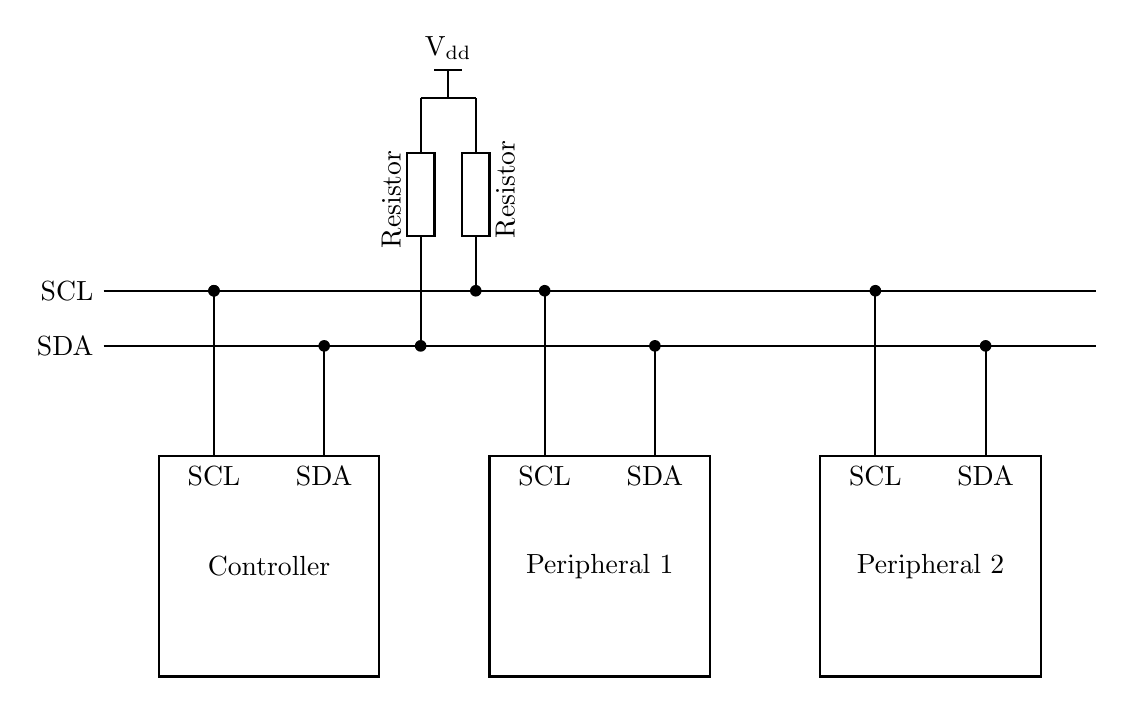
\begin{tikzpicture}[scale=0.7]
		% BLOCKS
		\draw[thick] (0,0) rectangle (4,4) node (dev1) [pos=0.5] {Controller};
		\draw[thick] (6,0) rectangle (10,4) node (dev2) [pos=0.5] {Peripheral 1};
		\draw[thick] (12, 0) rectangle (16,4) node (dev3) [pos=0.5] {Peripheral 2};
		\draw[thick] (4.5, 8) rectangle (5,9.5) node (r1) [above=2ex,pos=0.15, rotate=90] {Resistor};
		\draw[thick] (5.5, 8) rectangle (6,9.5) node (r2) [below=2ex,pos=0.85, rotate=90] {Resistor};
		
		% ARROWS	
		\draw [thick] (-1,6) node [anchor=east] {SDA} -- (17,6) ;
		\draw [thick] (-1,7) node [anchor=east] {SCL} -- (17,7)  ;
		\draw [thick] (1,4) node [anchor=north] {SCL} -- (1,7) ;
		\draw [thick] (3,4) node [anchor=north] {SDA} -- (3,6) ;
		\draw [thick] (7,4) node [anchor=north] {SCL} -- (7,7) ;
		\draw [thick] (9,4) node [anchor=north] {SDA} -- (9,6) ;
		\draw [thick] (13,4) node [anchor=north] {SCL} -- (13,7) ;
		\draw [thick] (15,4) node [anchor=north] {SDA} -- (15,6) ;
		\fill[black]  (1,7) circle (3pt) ;
		\fill[black]  (1,7) circle (3pt) ;
		\fill[black]  (7,7) circle (3pt) ;
		\fill[black]  (13,7) circle (3pt) ;
		\fill[black]  (3,6) circle (3pt) ;
		\fill[black]  (9,6) circle (3pt) ;
		\fill[black]  (15,6) circle (3pt) ;
		\draw [thick] (4.75,6)  -- (4.75,8) ;
		\fill[black]  (4.75,6) circle (3pt) ;
		\draw [thick] (5.75,7)  -- (5.75,8) ;
		\fill[black]  (5.75,7) circle (3pt) ;
		\draw [thick] (5.75,9.5)  -- (5.75,10.5) ;
		\draw [thick] (4.75,9.5)  -- (4.75,10.5) ;
		\draw [thick] (4.75,10.5)  -- (5.75,10.5) ;
		\draw [thick] (5.25,10.5)  -- (5.25,11) ;
		\draw [thick] (5,11)  -- node [above,pos=0.5] {V\textsubscript{dd}} (5.5,11) ;
	\end{tikzpicture}
	\label{fig:i2c}
	\caption{I\textsuperscript{2}C allows for multiple controllers and peripherals on the same bus.}
\end{figure}


\section{I2C}
I2C addresses for modules that are on the board or may be used with the board can be seen in Table \ref{table:i2caddresses}.

\begin{table}[!ht]
	\centering
	\begin{tabular}{l l}
		\hline
		Address (HEX) & Module \\ 
		\hline
		0x44 or 0x45 & SHT31-DIS Temperature/Humidity \\
		0x3D & 1.3" 128x64 OLED Display \\
		0x39 & APDS-9960 Light, Color, Proximity, Gesture \\
		0x77 & BME688 Temperature, Humidity, Gas \\
		0x2D, 0x53, and 0x57 & ST25DV16 Dynamic NFC/RFID Tag IC \\
		0x30 or other  & NeoKey 1x4 QT breakout board \\
		0x10 & STEMMA MiniGPS \\
		\hline
	\end{tabular}
	\caption{I2C addresses for relevant modules.}
	\label{table:i2caddresses}
\end{table}